%& -job-name=lesson1
\documentclass[10pt]{beamer}
%\documentclass[handout,10pt]{beamer}
%\mode<presentation>
%{
%  \usetheme{Berkeley}
%  \usecolortheme{seahorse}
%  \usefonttheme{default}  
%  \setbeamertemplate{navigation symbols}{}
%  \setbeamertemplate{caption}[numbered]
%} 

\usetheme{metropolis}

\usepackage[english]{babel}
\usepackage[utf8x]{inputenc}
\usepackage{caption}
\usepackage{multirow}
\usepackage{mathrsfs}
\usepackage{graphicx}
\usepackage{amsmath}
\usepackage{graphicx}
\usepackage[compatibility=false]{caption}
\usepackage{subcaption}
\usepackage[normalem]{ulem}
\DeclareMathOperator{\tr}{tr}
\usepackage{textpos}
\usepackage{animate}

\usepackage{tcolorbox}
\tcbset{colback=blue!5!white,colframe=blue!50!black}

\title[Computational Thinking]{Lesson 2: Number Systems}
%\titlegraphic{\includegraphics[height=1.57cm]{logo.jpg}}
\author[Scott Morgan]{\textbf{Scott Morgan}}
\institute{\textit{Bridgend College}
	\\
	\textit{BTEC Computing: Computational Thinking (Unit 18)} \\ \\ \\
	\textit{Web: scott3142.com} \\ 
	\textit{E-mail: MorganSN@cardiff.ac.uk}}
\date

\begin{document}

\begin{frame}
	\maketitle
	\begin{textblock*}{2cm}(7.5cm,-3cm)
		
\includegraphics[height=1.57cm]{bcoll_logo.png}
	\end{textblock*}
\end{frame}

\begin{frame}{Counting}
\begin{columns}	
	\begin{column}{0.5\textwidth}
		\begin{itemize}[<+->]
			\item Earliest evidence of counting dates back 35,000 years. Lines scratched on bone.
			\item Counting has evolved greatly since then.
		\end{itemize}
	\end{column}
	\begin{column}{0.5\textwidth}
	\begin{figure}[h]
		\centering
		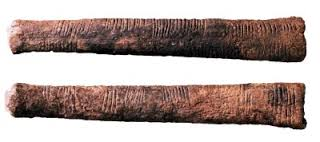
\includegraphics[scale=0.25]{bonecount.jpg}
		\caption*{}
	\end{figure}
\end{column}
\end{columns}
\end{frame}

\begin{frame}{The Number Line}
	\begin{figure}[h]
		\centering
		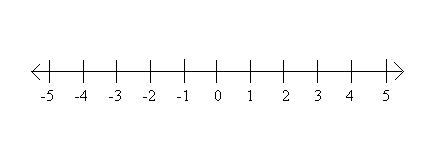
\includegraphics[scale=0.7]{numberline.png}
		\caption*{}
	\end{figure}
	\vspace{-10mm}
	\only<2->{
		\begin{figure}[h]
			\centering
			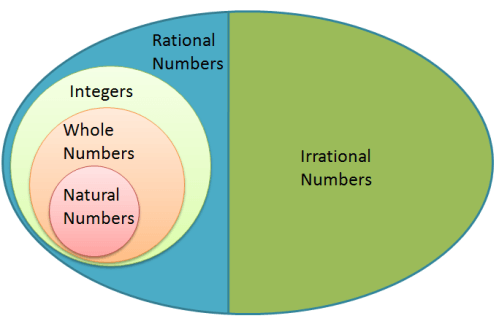
\includegraphics[scale=0.3]{numbers.png}
			\caption*{}
		\end{figure}
	}
\end{frame}

\begin{frame}{Base 10}
	\begin{itemize}[<+->]
		\item We all count with a number system called \textit{base 10}.
		\item This is probably because we have 10 fingers, which makes it easier.
		\item You can count in \textit{any other base}.
		\item What does this mean?
	\end{itemize}
\end{frame}

\begin{frame}{Review of Powers}
	\begin{itemize}[<+->]
		\item Evaluate the following:
		$$3^2 \only<2->{= 9}$$ 
		$$2^4 \only<3->{= 16}$$
		$$5^3 \only<4->{= 125}$$
		$$10^3 \only<5->{= 100}$$
		$$3\times10^5 \only<6->{= 30000}$$
		$$1^5 \only<7->{= 1}$$
		$$0^{53} \only<8->{= 0}$$
		$$345^0 \only<9->{= 1}$$
	\end{itemize}
\end{frame}

\begin{frame}{Revisit Base 10}
	\begin{itemize}[<+->]
		\item We can write any whole number as combinations of powers of 10s:
		\visible<2->{$$324 = \underbrace{(3\times10^2)}_{=300} + \underbrace{(2\times10^1)}_{=20} + \underbrace{(4\times10^0)}_{=4}$$}
		\visible<3->{$$3024 = \underbrace{(3\times10^3)}_{=3000} + \underbrace{(0\times10^2)}_{=0} + \underbrace{(2\times10^1)}_{=20} + \underbrace{(4\times10^0)}_{=4}$$}
		\visible<4->{$$1240 = \visible<5->{\underbrace{(1\times10^3)}_{=1000} + \underbrace{(2\times10^2)}_{=200} + \underbrace{(4\times10^1)}_{=40} + \underbrace{(0\times10^0)}_{=0}$$}}
		\visible<6->{$$1506 =  \visible<7->{\underbrace{(1\times10^3)}_{=1000} + \underbrace{(5\times10^2)}_{=500} + \underbrace{(0\times10^1)}_{=0} + \underbrace{(6\times10^0)}_{=6}$$}}
	\end{itemize}
\end{frame}

\begin{frame}{What about Base 2?}
	\begin{itemize}[<+->]
		\item We \textit{could} write any whole number as combinations of powers of 2s:
		\visible<2->{$$12_{10} = \underbrace{(1\times2^3)}_{=8} + \underbrace{(1\times2^2)}_{=4} + \underbrace{(0\times2^1)}_{=0} + \underbrace{(0\times2^0)}_{=0} = 1100_2$$}
		\visible<3->{$$18_{10} = \underbrace{(1\times2^4)}_{=16} + (0\times2^3)}_{=0} + \underbrace{(0\times2^2)}_{=0} + \underbrace{(1\times2^1)}_{=2} + \underbrace{(0\times2^0)}_{=0} = 10010_2$$}
	\end{itemize}
\end{frame}

\end{document}
